%! Author = Len Washington III
%! Date = 1/15/24

% Preamble
\documentclass[lab=1,title={Speaking rate},turnin=false]{com310lab}
\usepackage{amsmath}

% Document
\begin{document}

\maketitle

\begin{overview}
	Speaking rate refers to how fast or slow one speaks.
	For example, many people describe the variety of English from the rural American South as exhibiting a ``drawl'' that is characterized by slow speech, among other attributes.
	In contrast, speech from the urban North East is sometimes described as fast and under-articulated.
	In addition, the speech of women is often described as faster, compared to the speech of men.
	This claim about gender differences in speaking rate is seen not only in popular accounts of speech, but also in supposedly academic publications, e.g. Brizendine (2007), The Female Brain.
	(All of these claims, by the way, turn out to be false, but that’s another matter).
\end{overview}


\begin{problem}
	Various methods are used to measure speaking rate.
	One method estimates the number of words-per-minute of a speech sample, while another method estimates the number of syllables-per-second.
	They are calculated as follows:\\

	\begin{equation*}
	\begin{aligned}
		&\mbox{Words per minute} = \frac{\mbox{\# words in speech sample}}{\mbox{duration of speech sample, in seconds}} \times 60 \mbox{ seconds}\\
		&\mbox{Syllables per second} = \frac{\mbox{\# syllables in speech sample}}{\mbox{duration of speech sample, in seconds}}
	\end{aligned}
	\end{equation*}\\

	In theory, both methods should yield similar results: speech found to be fast using one method should also be seen as fast using the other.
	Your job is to determine whether this expectation is true and explain why.
\end{problem}

\begin{task}
	Record the paragraph below using any voice recorder app.
	For example, ``voice memos'' on an iPhone will work, so long as you are able to find start and end times for any sentence.
	If you prefer, you can also use any of the recorded files in the ``Lab 1 files'' folder from past students who have agreed to let other students use their files.
	\begin{displayquote}
		Today was busy with preparations.
		Many of the students collected several important statements.
		John gave the book to Mark then put the keys on the chair.
		Sally opened the closet and removed a sweater.
		Fred closed the door and left the room.
		Mary delivered the computer to Susan then handed the papers to the teacher.
		All of the class had lots of things to do.
		Eventually, everyone completed the task they needed to perform.
	\end{displayquote}
	Then, compute the speaking rate for each sentence, using both words-per-minute (w.p.s.) and syllables-per-second (s.p.s) for each sentence as described above.
	You need no special tools to count the number of words and syllables in each sentence.
	If you need help with counting syllables, consult any dictionary--wiktionary is fine.
	To measure the duration of the speech sample, open the recording of your file, delete any pauses or false starts, and then select one sentence at a time and note its duration in seconds.
	Now, examine differences across certain sentences.
	For the purposes of this lab, ignore the first and last sentences.
	The other sentences are numbered as follows:
	\begin{displayquote}
		Sentence 1: Many of the students$\dots$\\
		Sentence 2: John gave$\dots$\\
		Sentence 3: Sally opened$\dots$\\
		Sentence 4: Fred closed$\dots$\\
		Sentence 5: Mary delivered$\dots$\\
		Sentence 6: All of$\dots$\\
	\end{displayquote}
	Compare w.p.m.\ and s.p.s.\ for the odd-numbered sentences to the same measures for the even-numbered sentences.
	Generate a table or graph showing your results.
	Summarize the results, and address the problem raised above, namely whether measures of speaking rates are consistent.
	If you find any differences, use the data to offer an explanation.
	(Hint: the measures are unlikely to be consistent with each other).
\end{task}

\begin{writeup}
	Follow the format for writing up phonetics lab reports and turn in your report on the day it is due.
\end{writeup}

\pagebreak

\labtitle

\begin{topic}
	Clearly state the topic that you are investigating.
	An example would be, ``This lab addresses the way adults talk to pets versus infants.''
\end{topic}

\begin{issue}
	A description of the issue at stake.
	An issue is the problem that you are attempting to solve.
	An example would be,
	``The special register of infant-directed speech is sometimes claimed to be intended to clearly convey speech characteristics to language-learning infants, yet speech to pets would appear to share this same special register, and there is no suggestion that adults talk to pets in this way to help them learn language.
	At issue is whether pet- and infant-directed speech are, in fact, identical.''
	You need only cite relevant information from our lectures, from the textbook, or from the lab instructions itself to motivate your issue, but however you decide to state the issue, be clear to draw out what is at state in addressing it.
\end{issue}

\begin{hypothesis}
	A statement of the research questions and hypotheses under investigation.
	A hypothesis is a tentative explanation for an (anticipated) observation of data.
	An example would be, ``Data were analyzed to address the issue of pet- vs. infant-directed speech.
	I predict that if speech directed to infants is intended to be clear, then such speech would have, among other properties, an expanded vowel space because xxx.
	In contrast, if pet-directed speech is diminutive and not intended for language-learning purposes, then such speech would be characterized as being merely loud speech and not show any expanded vowel space because yyy.''
	This particular hypothesis requires quite a bit of knowledge of phonetics, which you will not possess at the beginning of the semester.
	You should state a hypothesis as strongly as your knowledge of phonetics and speech characteristics allow.
	Don’t go out on a limb and guess at things if you are uncertain.
\end{hypothesis}

\begin{method}
	A description of the method.
	An example would be,
	``In the lab activity, I recorded x people saying y words to z pets, and then the same x people saying the same words to z infants.
	Then, I made the following measurements: x, y, and z.''
	Be specific.
	Explain what equipment you used, or how data were obtained.
	Define any measurements.
	An example would be,
	``Loud speech was defined as any speech with an average intensity of xxx, and expanded vowel space was defined as cases where [acoustic measures] showed yyy.''
\end{method}

\begin{results}
	A description of the results.
	An example would be,
	``Results indicated vowel space for pet-directed speech exhibited louder, longer segments, but not a bigger vowel space, consistent with the prediction that such speech is merely loud and not meant to help discriminate among speech sounds.
	In contrast, infant directed speech did exhibit an expanded vowel space, which I take as evidence as supporting the hypothesis that the special register to infants is for language learning purposes and is acoustically distinct from pet-directed speech.''
	Provide relevant tables, figures of (minimally) descriptive statistics where relevant.

	\makebox[1 \textwidth][c]{
		\newcolumntype{C}[1]{>{\centering\arraybackslash}p{#1\textwidth}}
			\begin{threeparttable}
				\caption{Results from the Lab}
				\label{tab:data}
				\begin{tabular}{|C{0.1}C{0.2}C{0.15}C{0.15}C{0.23}C{0.23}|}
	\hline
	Sentence Number&Sentence Duration (s)&Words per Sentence&Syllables per Sentence&Words per Minute (w.p.m)&Syllables per Seconds (s.p.s)\\
0&2.950393&5&10&101.6813692277605&3.3893789742586833\\
1&3.734091&8&16&128.54534075361315&4.284844691787105\\
2&3.826291&13&13&203.85276498833989&3.397546083138998\\
3&3.641891&8&13&131.79966121995412&3.5695741580404245\\
4&3.088693&8&8&155.40553884766146&2.590092314127691\\
5&5.393687&13&22&144.61350834781476&4.078842543143494\\
6&2.443294&10&10&245.5701196826907&4.092835328044845\\
7&3.964591&9&19&136.2057271481472&4.792423732990364\\
\hline\end{tabular}
%				\begin{tablenotes}
%					\small
%					\item
%				\end{tablenotes}
			\end{threeparttable}
	}

	\begin{figure}[H]
		\centering
		\caption{A scatter plot showing the words per minutes against the syllables per second of \hyperref[tab:data]{sentences} 1--6.}
		\label{fig:results}
		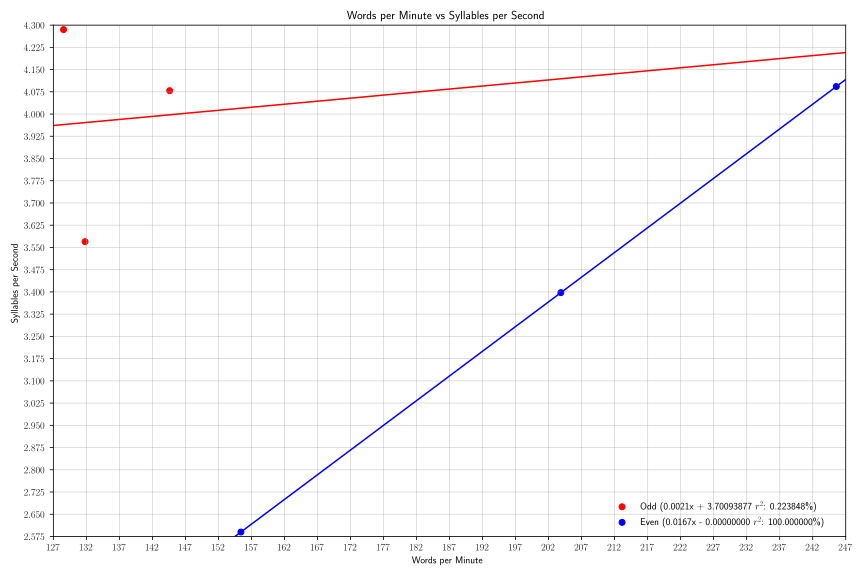
\includegraphics[width=\textwidth]{washington_lab1_graph}
	\end{figure}
\end{results}

% TODO: Discuss how the even sentences have the same number of syllables as words, whereas the odds don't. For the 1:1 syllable:word ratio sentences, the slope is seems about 1 (use washmath to find the actual slope), whereas the odd sentences vary due to the different rations for each sentence, however, there seems to be a 1:2 ratio of words:syllables, which would track if sentence 3 wasn't an outlier.
\begin{discussion}
	A critical analysis of your study.
	An example would be,
	``While the study revealed a difference in pet- versus infant-directed speech, it does have some drawbacks.
	First, I didn't discuss whether infant-directed speech is actually effective in helping infants to discriminate among speech sounds.
	Moreover, vowel-space isn’t necessarily a strong indicator of an attempt to teach an infant to discriminate among speech sounds in the first place. Rather, an equally plausible explanation could be that adults xxx.''
\end{discussion}

\end{document}